$$E(s)=R(s)-Y(s)$$
Donde: E(s) es el error medido, R(s) es la referencia y Y(s) es la salida.
$$H(s)=frac{Y(s)}{X(s)}$$
$$Y(s)=H(s)KX(s)$$
Si E(s)=X(s):
$$Y(s)=H(s)KE(s)$$
$$Y(s)=\frac{1}{s(s+3)}KE(s)$$
$$Y(s)=\frac{KE(s)}{s(s+3)}$$
$$E(s)=\frac{Y(s)(s(s+3))}{k}$$
Si $E(s)=R(s)-Y(s)$
$$R(s)-Y(s)=\frac{Y(s)(s(s+3))}{k}$$
$$KR(s)-KY(s)=Y(s)(s(s+3))$$
$$KR(s)=Y(s)(s(s+3)+K)$$
$$G_{c}(s)=\frac{Y(s)}{R(s)}=\frac{K}{s(s+3)+K}$$
Función de transferencia de lazo cerrado:
$$G_{c}(s)=\frac{Y(s)}{R(s)}=\frac{K}{(s(s+3)+K)}$$	
Si k=1:
$$G(s)=\frac{1}{(s(s+3)+1)}$$	
$$G(s)=\frac{1}{s^{2}+3s+1}$$	

\begin{figure}[H]
	\centering
	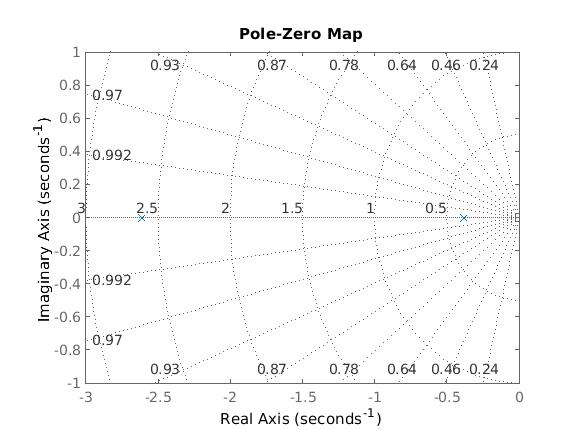
\includegraphics[scale=0.5]{G3.jpg}\
	\caption{{Si K=1}}
	\label{fig:salidaTs001-6}
\end{figure}
Polos: $P_{1}=-2.618$ y $P_{2}=-0.382$. Por lo tanto es estable el sistema.\\
Respuesta al escalón del sistema:\\

\begin{figure}[H]
	\centering
	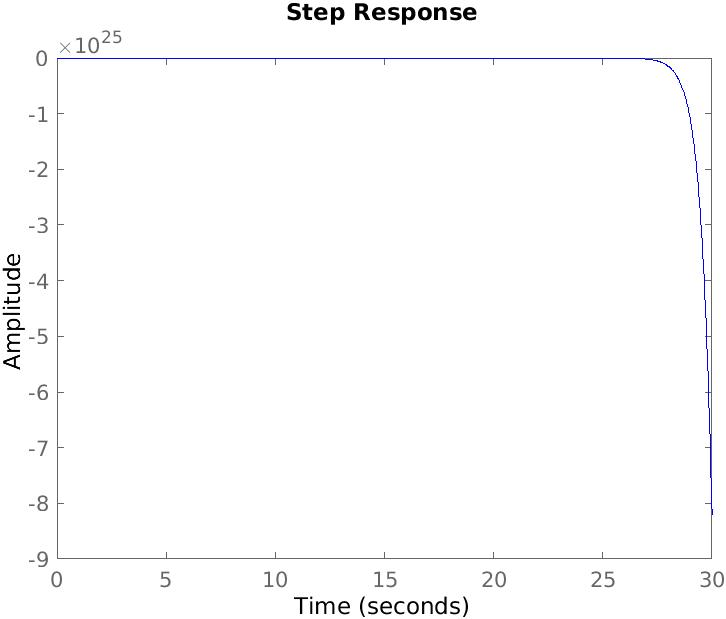
\includegraphics[scale=0.4]{G6.jpg}
	\caption{{Respuesta al escalón del sistema}}
	\label{fig:salidaTs001-6}
\end{figure}


Si k=-10:
$$G(s)=\frac{-10}{(s(s+3)-10)}$$	
$$G(s)=\frac{-10}{s^{2}+3s-10}$$

\begin{figure}[H]
	\centering
	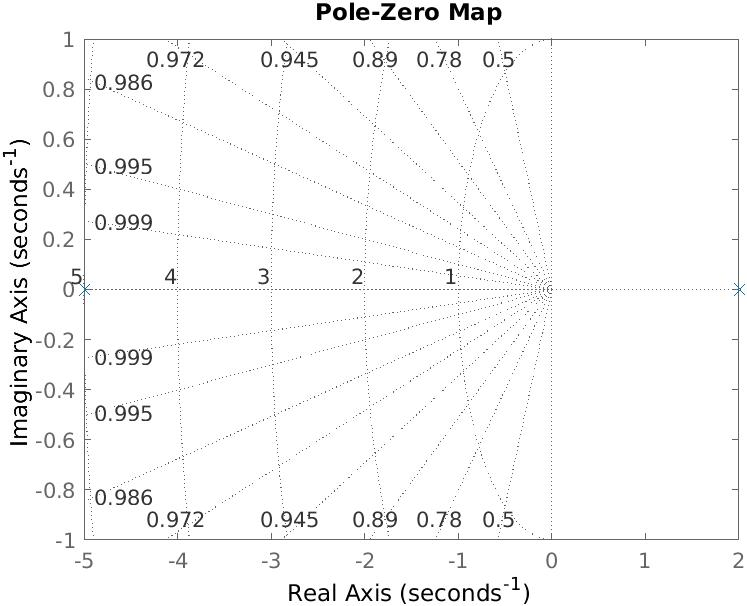
\includegraphics[scale=0.36]{G4.jpg}
	\caption{{Si K=-10}}
	\label{fig:salidaTs001-6}
\end{figure}


Polos: $P_{1}=-5$ y $P_{2}=2$. Por lo tanto es inestable el sistema.\\
Respuesta al escalón del sistema:

\begin{figure}[H]
	\centering
	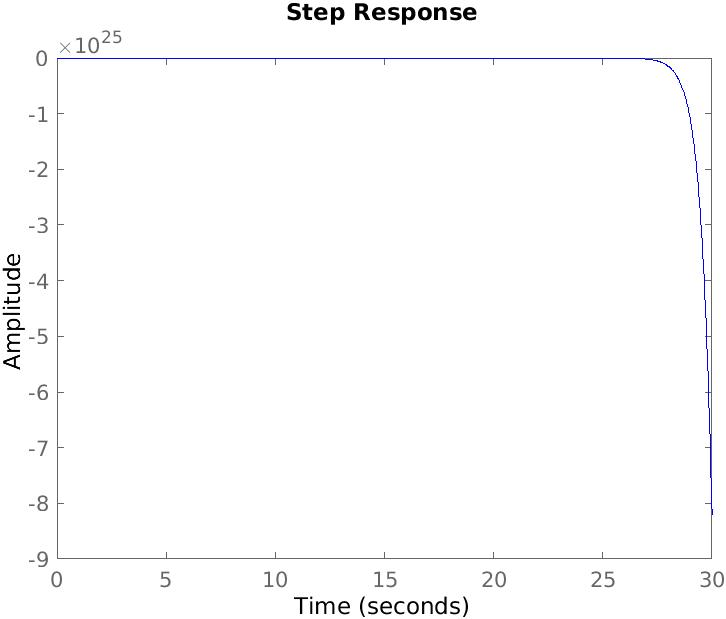
\includegraphics[width=0.4\linewidth]{G6.jpg}
	\caption{{Respuesta al escalón del sistema}}
	\label{fig:salidaTs001-7}
\end{figure}